\uchapter{\ChapterTitleAppendix}
\label{sec:appendix}

\section*{Szczegóły implementacji algorytmu Gumbel AlphaZero}

\begin{algorithm}
    \caption{Pętla główna uczenia AlphaZero}\label{alg:alphazero-main}
    \KwOut{Learned weights $\theta$}
    $\theta \gets$ initial random weights\;
    Collect observations from random-move games to initialize batch norm stats\;
    experience\_buffer $\gets$ empty list\;
    \Repeat{training budget exhausted}{
        \For{$i \gets 1$ \KwTo self-play games per epoch}{
            $T \gets$ self\_play($\theta$)\;
            $X \gets$ process\_trajectory($T$)\;
            experience\_buffer $\gets$ experience\_buffer $\cup$ $X$\;
        }
        Truncate experience\_buffer to fixed size with most recent data\;
        \For{$i \gets 1$ \KwTo training iterations}{
            $X \gets$ sample batch from experience\_buffer without replacement\;
            $\theta \gets$ train\_step($\theta$, $X$)\;
        }
    }
    \Return $\theta$\;
\end{algorithm}

\begin{algorithm}
    \caption{Procedura self\_play}\label{alg:alphazero-self-play}
    \KwIn{Weights $\theta$}
    \KwOut{Trajectory $T$}
    $T \gets$ empty list\;
    $s \gets$ random initial game state\;
    \While{$s$ is not terminal}{
        \tcc{See algorithm in \cite{GumbelAZ}}
        $\pi \gets$ GumbelAlphaZeroPolicy($s$, $\theta$)\;
        $a \gets$ GumbelRootActionSelection($\pi$)\;
        $s' \gets$ $s$.apply($a$)\;
        $s$.action\_weights $\gets$ $\pi$\;
        $T \gets T \cup \{s\}$\;
        $s \gets s'$\;
    }
    \Return $T$\;
\end{algorithm}

\begin{algorithm}
    \caption{Procedura process\_trajectory}\label{alg:alphazero-process-trajectory}
    \KwIn{Trajectory $T$}
    \KwOut{Batch of training data $X$}
    $X \gets$ empty list\;
    \ForEach{state $s$ in $T$}{
        $x \gets$ empty example\;
        $x$.observation $\gets$ $s$.observation\;
        $x$.policy\_target $\gets$ $s$.action\_weights\;
        $x$.value\_mask $\gets$ $1$ if $T[\mathrm{end}]$ is terminal, $0$ otherwise\;
        $x$.value\_target $\gets \begin{cases}
                1  & \text{if}\ T[\mathrm{end}].\mathrm{winner} = s.\mathrm{player}                 \\
                -1 & \text{if}\ T[\mathrm{end}].\mathrm{winner} = \mathrm{other}(s.\mathrm{player}) \\
                0  & \text{otherwise}
            \end{cases}$\\
        $X \gets X \cup \{x\}$\;
    }
    \Return $X$\;
\end{algorithm}

\begin{algorithm}
    \caption{Procedura train\_step}\label{alg:alphazero-train-step}
    \KwIn{Weights $\theta$, batch of training data $X$}
    \KwOut{Updated weights $\theta$}
    \ForEach{example $x$ in $X$}{
        $z \gets$ $x$.value\_target\;
        $m \gets$ $x$.value\_mask\;
        $\pi \gets$ $x$.policy\_target\;
        $v, \mathbf{p} \gets$ model($x$.observation, $\theta$)\;
        $\mathcal{L} \gets m(z - v)^2 - \pi^T \log \mathbf{p} + c ||\theta||^2$\;
        $\theta \gets$ adam\_optimizer\_step($\theta$, $\mathcal{L}$)\;
    }
    \Return $\theta$\;
\end{algorithm}

\begin{table}
    \centering
    \caption{Parametry algorytmu Gumbel AlphaZero}
    \label{tab:gumbel-alphazero-params}
    \begin{tabular}{ll}
        \toprule
        Parametr & Wartość \\ \midrule
        Gumbel scale \cite{GumbelAZ} & 1.0 \\
        MCTS max depth & 64 \\
        MCTS simulations & 32 \\
        $Q$-value transform & Completed by mix value \cite{GumbelAZ}; Appendix D \\
        Self-play iterations per epoch & 8 \\
        Self-play batch size & 256 \\
        Training iterations per epoch & 16 \\
        Training batch size & 8192 \\
        Experience buffer size & 1e6 \\
        Optimizer & Adam \cite{Adam} \\
        Learning rate & 1e-3 \\
        Regularization constant $c$ & 1e-4 \\
        Epochs & 846 \\
        Training time & 21h 26m \\
        \bottomrule
    \end{tabular}
\end{table}

\begin{table}
    \centering
    \caption{Architektura sieci neuronowej}
    \label{tab:nn-architecture}
    \begin{tabular}{ll}
        \toprule
        Warstwa & Rozmiar \\ \midrule
        Input & (480) \\
        Linear & (4, 4, 32) \\
        \midrule
        \multicolumn{2}{c}{Initial convolution} \\
        Conv2D 3x3 & (4, 4, 64) \\
        BatchNorm & (4, 4, 64) \\
        ReLU & (4, 4, 64) \\
        \midrule
        \multicolumn{2}{c}{Residual block $\times 9$} \\
        Conv2D 3x3 & (4, 4, 64) \\
        BatchNorm & (4, 4, 64) \\
        ReLU & (4, 4, 64) \\
        Conv2D 3x3 & (4, 4, 64) \\
        BatchNorm & (4, 4, 64) \\
        Residual connection & (4, 4, 64) \\
        ReLU & (4, 4, 64) \\
        \midrule
        \multicolumn{2}{c}{Policy head} \\
        Conv2D 1x1 & (4, 4, 2) \\
        BatchNorm & (4, 4, 2) \\
        ReLU & (4, 4, 2) \\
        Linear & (38) \\
        \midrule
        \multicolumn{2}{c}{Value head} \\
        Conv2D 1x1 & (4, 4, 1) \\
        BatchNorm & (4, 4, 1) \\
        ReLU & (4, 4, 1) \\
        Linear & (256) \\
        ReLU & (256) \\
        Linear & (1) \\
        Tanh & (1) \\
        \bottomrule
    \end{tabular}
\end{table}

\FloatBarrier

\section*{AlphaZero i gry z niepełną informacją}

W pracy kluczowym aspektem okazała się teoria gier, która pozwoliła na
formalną weryfikację zastosowanych algorytmów.
Kluczowymi aspektami gier są: liczba graczy, determinizm,
specyfikacja nagrody oraz informacja dostępna graczom.
Udało się poprawnie pod względem teoretycznym poradzić sobie
z~pierwszymi trzema aspektami, jednakże ostatni okazał się
problematyczny.

\subsection*{MiniMax a stan równowagi Nasha}

Podstawowe nasze założenie polegało na tym, że
sieć neuronowa, poprzez aproksymację algorytmu MCTS,
będzie dążyć do strategii MiniMax.
Zostało to udowodnione w rozdziale \nameref{sec:wybrane-aspekty-realizacji}.
Jest to jednak MiniMax dla wariantu brydża z~pełną informacją,
kiedy gracze, czyli algorytm, widzi wszystkie karty.
\\
\textbf{Nawet jeśli sieć nie widzi wszystkich kart,
to aproksymuje algorytm, który to robi.}
\\
MiniMax wybiera ruch, który minimalizuje maksymalną możliwą stratę.
Strategia MiniMax dla gier o~sumie zerowej i~pełnej informacji
jest stanem równowagi Nasha.
Stan równowagi Nasha to strategia, od której odstąpienie
nie przynosi żadnemu z graczy korzyści, pod warunkiem,
że pozostali gracze nie zmieniają swoich strategii.
Odnalezienie stanu równowagi Nasha dla brydża z~niepełną informacją
byłoby strategią idealną i~odkryciem naukowym stulecia.
Sama aproksymacja tej strategii byłaby graczem na poziomie mistrza.
\\
\textbf{MiniMax dla gier z~niepełną informacją nie musi być stanem równowagi Nasha}.
\\
To nieintuicyjne stwierdzenie oznacza, że AlphaZero nie ma gwarancji
poprawnego procesu uczenia w~brydżu.
Nasza implementacja opiera się na obserwacji, że w~praktyce
strategia osiągana przez sieć neuronową jest zadowalająco dobra.

\subsection*{Gra z Diabełkiem}

Przedstawiamy abstrakcyjną grę, ilustrującą powyższy problem.
Niech Diabełek i Człowiek będą graczami.
Diabełek ma olbrzymią dzidę, a~Człowiek ma mały miecz.
Diabełek i~Człowiek stoją naprzeciwko siebie.
Diabełek może wykonać jeden z~dwóch ruchów:
\begin{itemize}
    \item skierować dzidę w~lewo (akcja A),
    \item skierować dzidę w~prawo (akcja B).
\end{itemize}
Człowiek może wykonać analogiczne ruchy:
\begin{itemize}
    \item zaatakować Diabełka od lewej (akcja A),
    \item zaatakować Diabełka od prawej (akcja B).
\end{itemize}
Jeśli Diabełek i~Człowiek wykonają akcje w~tę samą stronę,
to Człowiek zostanie trafiony przez dzidę i~przegra.
Jeśli Diabełek i~Człowiek wykonają akcje w~przeciwne strony,
to Diabełek zostanie trafiony przez miecz i~przegra.
Akcje wykonywane są jednocześnie.
Aby zmienić balans akcji A/B, po stronie prawej (B)
umieszczone są przeszkody, które utrudniają atakowanie od prawej.
Tabela \ref{tab:devil-game-rewards} przedstawia nagrody
dla wszystkich możliwych kombinacji akcji.

\begin{table}
    \centering
    \caption{Nagrody w grze z Diabełkiem}
    \label{tab:devil-game-rewards}
    \begin{tabular}{llll}
        \toprule
        Akcja Diabełeka & Akcja Człowieka & Nagroda Diabełka & Nagroda Człowieka \\ \midrule
        A               & A               & 1                & -1                \\
        A               & B               & -0.5             & 0.5               \\
        B               & A               & -1               & 1                 \\
        B               & B               & 1                & -1                \\
        \bottomrule
    \end{tabular}
\end{table}


Dla potrzeb formalnych grę można zamienić na równoważną grę
sekwencyjną, w~której Diabełek wykonuje ruch pierwszy.
Człowiek nie zna akcji Diabełka, dlatego
jest to gra z~niepełną informacją.
Rys.~\ref{fig:devil-game-tree} przedstawia rozwiązanie MiniMax gry.
Wartości stanów $s_3$, $s_4$, $s_5$ i~$s_6$ to nagrody $r$
stanów terminalnych na podstawie Tab.~\ref{tab:devil-game-rewards}.
Wartości stanów $s_1$ i~$s_2$ to $\min(r(s_3), r(s_4))$ i~$\min(r(s_5), r(s_6))$.
Wartość stanu $s_0$ to $\max(r(s_1), r(s_2))$, czyli $-0.5$.
Oznacza to, że Diabełek nie jest w~stanie uzyskać nagrody większej niż $-0.5$.
Jeśli wybierze akcję A, to Człowiek wybierze akcję B i~Diabełek otrzyma nagrodę $-0.5$.
Jeśli wybierze akcję B, to Człowiek wybierze akcję A i~Diabełek otrzyma nagrodę $-1$.
Stanem równowagi Nasha jest zatem wybór akcji A przez Diabełka
oraz akcji przeciwnej przez Człowieka, ale tylko jeśli Człowiek
zna strategię Diabełka.

Teraz widoczne jest, dlaczego powyższa strategia nie działa
w~wersji Gry z~Diabełkiem z~niepełną informacją.
Jeśli Diabełek wybierze jednak akcję B, a Człowiek założy, że Diabełek
podążał strategią MiniMax, to wybierze akcję B i~przegra z~Diabełkiem.
Ponieważ Diabełek może zyskać zmianą strategii, to nie jest to stan równowagi Nasha.
Stanem równowagi Nasha dla tej gry jest losowanie akcji przez obu
graczy z~pewnym prawdopodobieństwem, maksymalizując wartość
oczekiwaną nagrody w~perspektywie wielu gier.

\begin{figure}
    \centering
    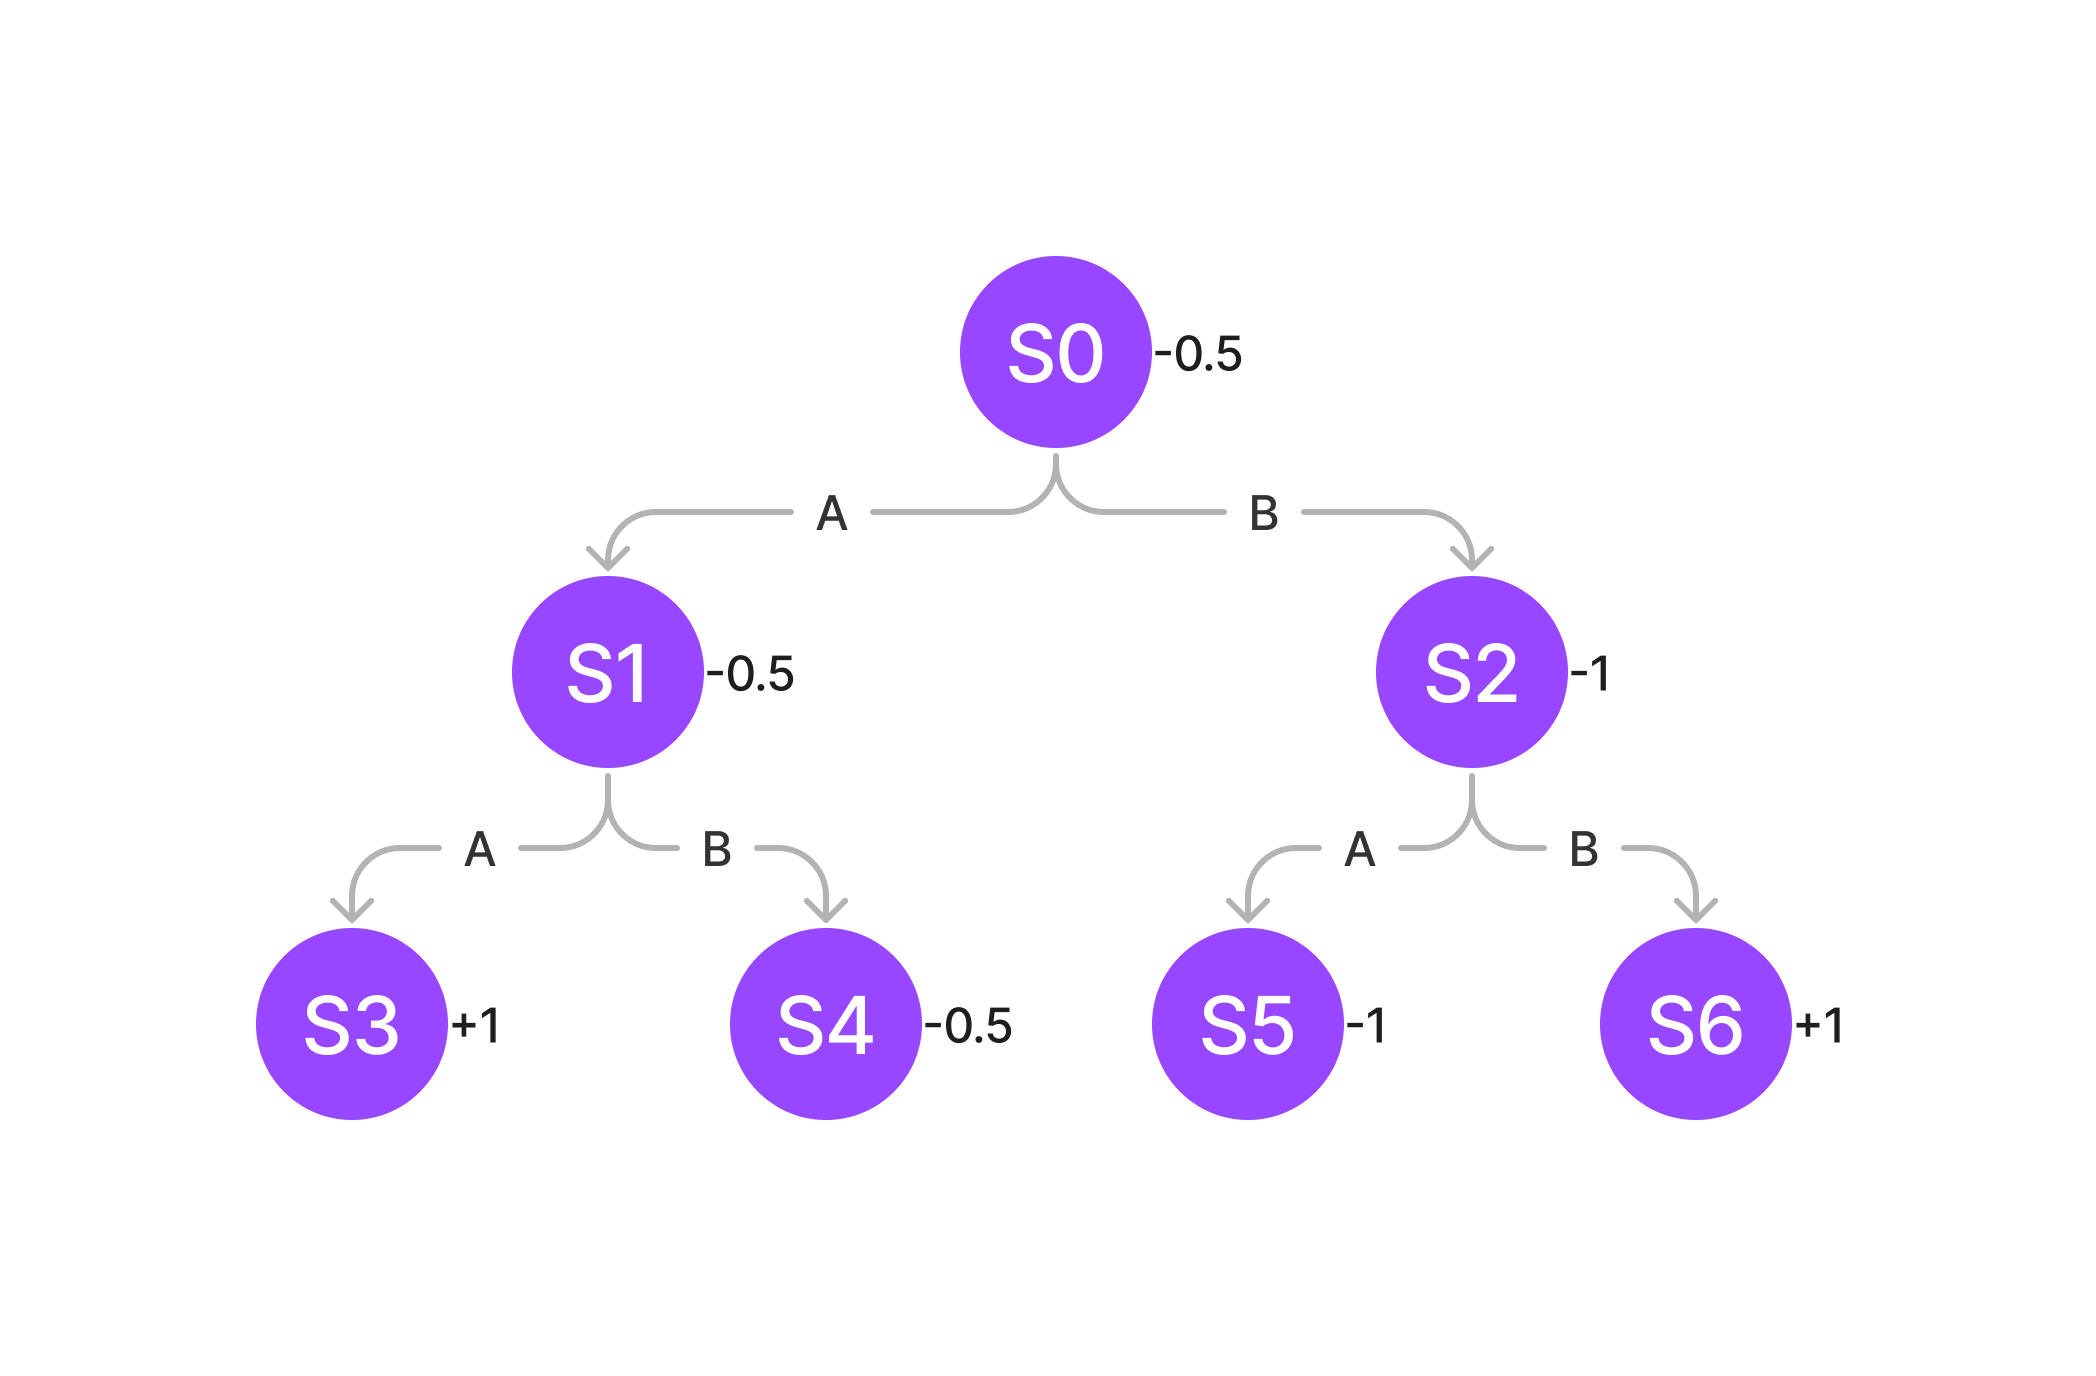
\includegraphics[width=\textwidth]{img/ai/devil-game-tree.png}
    \caption{Drzewo Gry z Diabełkiem.}
    \label{fig:devil-game-tree}
\end{figure}

\subsection*{Eksperymenty}

W celu zbadania powyższych rozważań przeprowadziliśmy eksperymenty
na Grze z~Diabełkiem.
Zaimplementowano grę zgodnie z~opisem powyżej
i~zastosowano algorytm AlphaZero.
Obserwacją była jedna wartość: czy gracz jest Diabełkiem, czy Człowiekiem.
Nauczoną sieć~$\mathbf{p}$ przedstawia Tab.~\ref{tab:devil-game-policy}.
Widać zbieżność $\operatorname{argmax} \mathbf{p}$ do strategii MiniMax.
Widać również, że sieć nauczyła się całkowicie przewidywalnej strategii,
która nie jest stanem równowagi Nasha.
Eksperyment potwierdza, że AlphaZero nie zawsze znajduje stan równowagi Nasha.
Pokazuje również, że sieć może nauczyć się strategii MiniMax,
co jest pozytywnym wynikiem.

\subsection*{Wnioski}

Wnioskowanie formalne jak i~wyniki eksperymentów pokazują,
że AlphaZero nie jest idealnym algorytmem do gier z~niepełną informacją.
W~naszej opinii, przez wysoki poziom skomplikowania gry w~brydża,
strategia osiągana przez AlphaZero wystarcza do pokonania mało doświadczonych graczy.
Wątpliwe jest jednak, aby algorytm osiągnął poziom mistrzowski.
W~przyszłości planowane jest zbadanie innych algorytmów,
lepiej przystosowanych do gier z~niepełną informacją,
na przykład Regularized Nash Dynamics \cite{doi:10.1126/science.add4679},
który ma gwarancję zbieżności do stanu równowagi Nasha.


\begin{table}
    \centering
    \caption{Nauczona funkcja polityki $\mathbf{p}$}
    \label{tab:devil-game-policy}
    \begin{tabular}{lll}
        \toprule
        Gracz & $\mathbf{p}_\mathrm{A}$ & $\mathbf{p}_\mathrm{B}$ \\ \midrule
        Diabełek & 1.0 & 0.0 \\
        Człowiek & 0.14 & 0.86 \\
        \bottomrule
    \end{tabular}
\end{table}


% 0 -> 0 = 1
% 0 -> 1 = -0.5
% 1 -> 0 = -1
% 1 -> 1 = 1

% Wins: 0.53, Draws: 0.00, Losses: 0.47
% [[1.         0.        ]
%  [0.14       0.85999995]]
